In section 2.2.1 categories of medical smart phone apps were defined. Apps in the same categories might have a similar feature set and capabilities. An app in the \textit{Alert / First Response} category might have a database that stores important contacts in the user’s area and a user interface that allows the user to quickly alert a contact in an emergency situation. An app in the \textit{Learning / Educational / Reference} category might be modelled as a quiz app which presents the user with a question and several possible answers to choose from. Answers from several questions will can be evaluated and a score is presented to the user at the end of a session. The app would be implemented with a database of questions and weighted answers, as well as an interface that presents the questions to the user sequentially.

One of the goals of this project is to define requirements for an app that provides a risk assessment of a lesion being benign or malignant. A high level description of the primary function of the app is the following:

\begin{itemize}[label={}]
\item The smart phone app allows the user to capture and analyse an image of a skin lesion and provide a risk assessment to the user of the lesion being a malignant melanoma.

\end{itemize}

The user might also like to save the image and results in oder to be able to compare it with other assessments in the future, or to review the assessment with a dermatologist. For comparison it might be useful to save associated metadata, such as the date and location on the body of the lesion. For convenience it might be nice to send the assessment and image via email to a specialist for review.
Secondary functionality can be described as follows:

\begin{itemize}[label={}]
\item The app allows the user to save or archive the image and corresponding assessment for future comparison and review.
\item The user can add, edit, and save metadata associated with the image of the lesion.
\item The user can browse archived images, assessments, and associated metadata.
\item The user can send a set of images with associated assessment and metadata via email.
\end{itemize}

From this high level description some basic assumptions about the app’s architecture can already be made. The app will require access to a database that can store information about an image, results of the analysis, and metadata. The app will require a user interface that allows a user to browse and edit data associated with an image. The app requires access to the smart phone’s camera api in order to capture images.
Another consideration that will impact design decisions is the investment already made in developing the image processing and analysis algorithms. Choosing python as the basis for the numerical algorithms and leveraging python based scientific computing libraries has implications because python code is not easily portable to iOS or Android devices. In order to efficiently utilise the algorithms as they are, and to continue to update and improve them, the image processing and analysis algorithms should be implemented as online services.

\begin{itemize}[label={}]
\item The image processing and risk assessment algorithms will be implemented as online services.
\end{itemize}

In order to formally elicit the requirements the hight level description will be broken down into structured use cases. A set of requirements will be extracted from the use cases.

\section{Use Cases}
        \begin{table}[H]
            \centering
            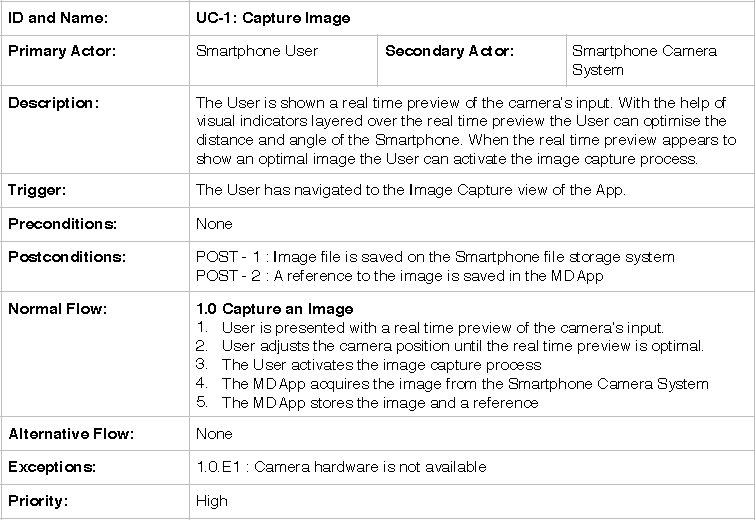
\includegraphics[width=\textwidth]{assets/requirements/uc/usecase_01.pdf}
            \caption{UC-1}
            \label{fig:uc-1}
        \end{table}
        \begin{table}[H]
            \centering
            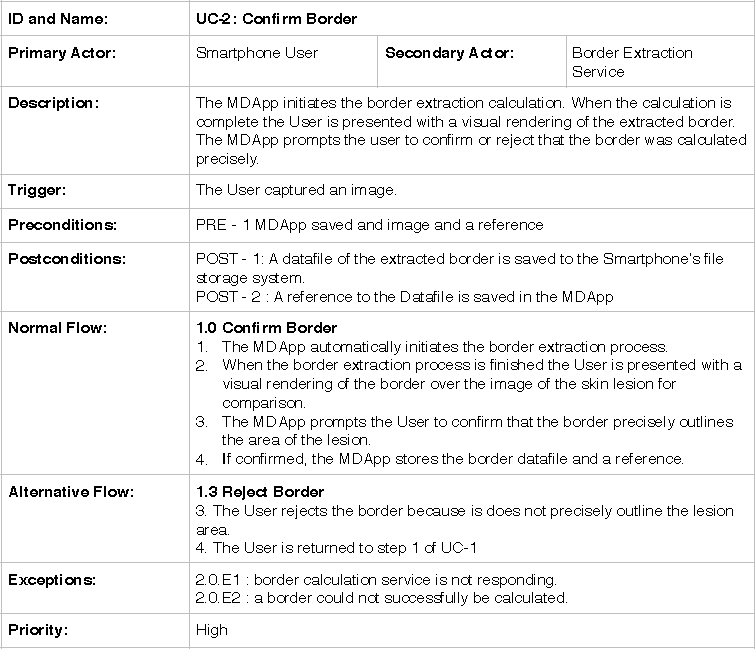
\includegraphics[width=\textwidth]{assets/requirements/uc/usecase_02.pdf}
            \caption{UC-2}
            \label{fig:uc-2}
        \end{table}
        \begin{table}[H]
            \centering
            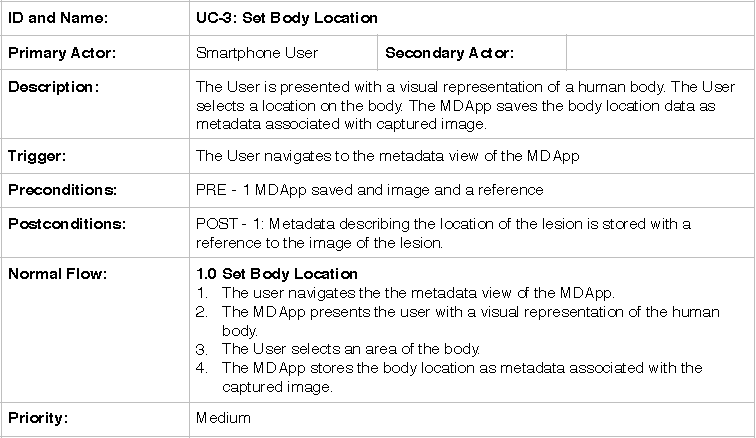
\includegraphics[width=\textwidth]{assets/requirements/uc/usecase_03.pdf}
            \caption{UC-3}
            \label{fig:uc-3}
        \end{table}
        \begin{table}[H]
            \centering
            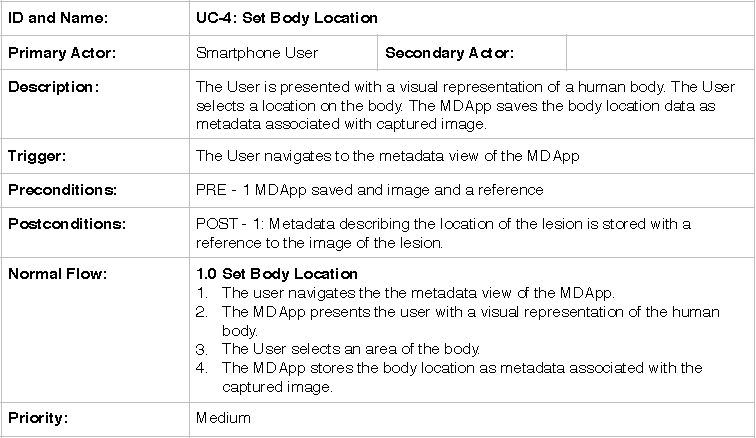
\includegraphics[width=\textwidth]{assets/requirements/uc/usecase_04.pdf}
            \caption{UC-4}
            \label{fig:uc-4}
        \end{table}
        \begin{table}[H]
            \centering
            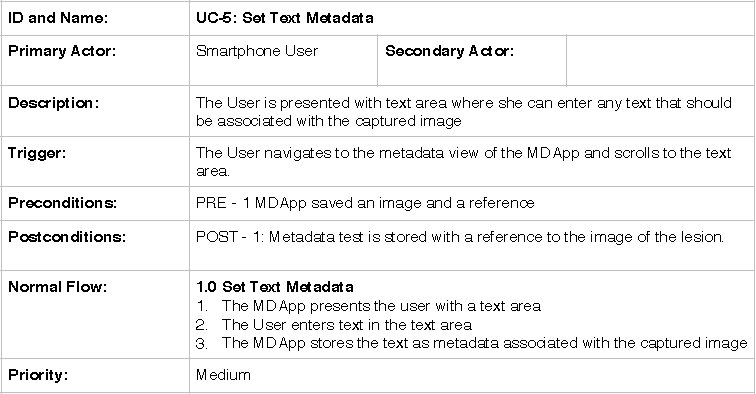
\includegraphics[width=\textwidth]{assets/requirements/uc/usecase_05.pdf}
            \caption{UC-5}
            \label{fig:uc-5}
        \end{table}
        \begin{table}[H]
            \centering
            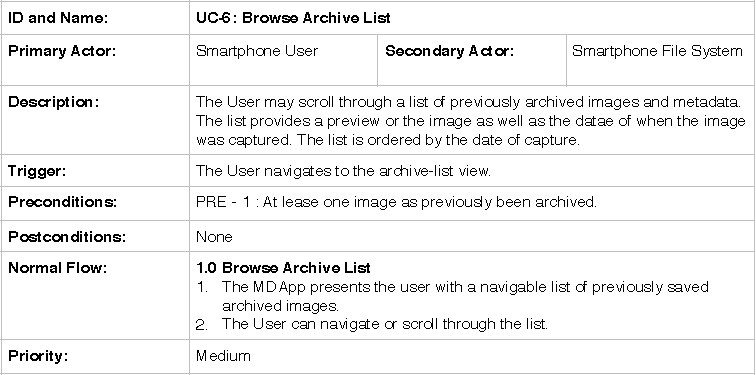
\includegraphics[width=\textwidth]{assets/requirements/uc/usecase_06.pdf}
            \caption{UC-6}
            \label{fig:uc-6}
        \end{table}
        \begin{table}[H]
            \centering
            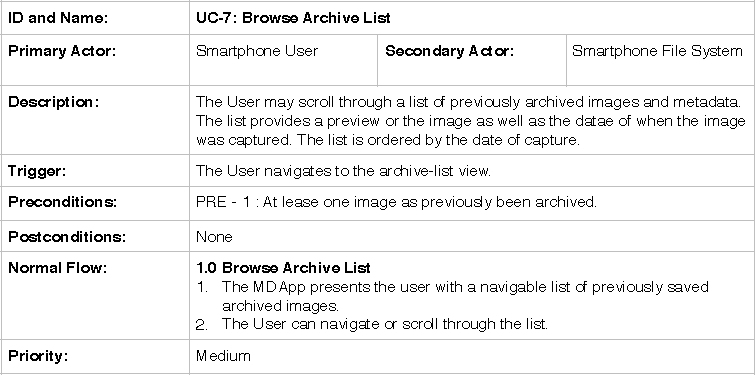
\includegraphics[width=\textwidth]{assets/requirements/uc/usecase_07.pdf}
            \caption{UC-7}
            \label{fig:uc-7}
        \end{table}
        \begin{table}[H]
            \centering
            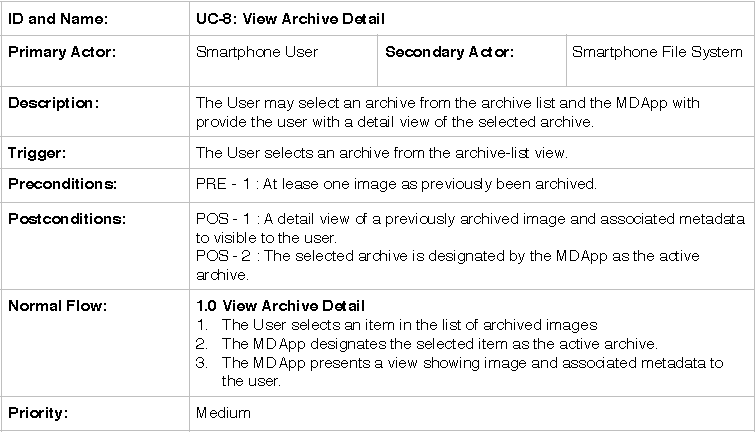
\includegraphics[width=\textwidth]{assets/requirements/uc/usecase_08.pdf}
            \caption{UC-8}
            \label{fig:uc-8}
        \end{table}
        \begin{table}[H]
            \centering
            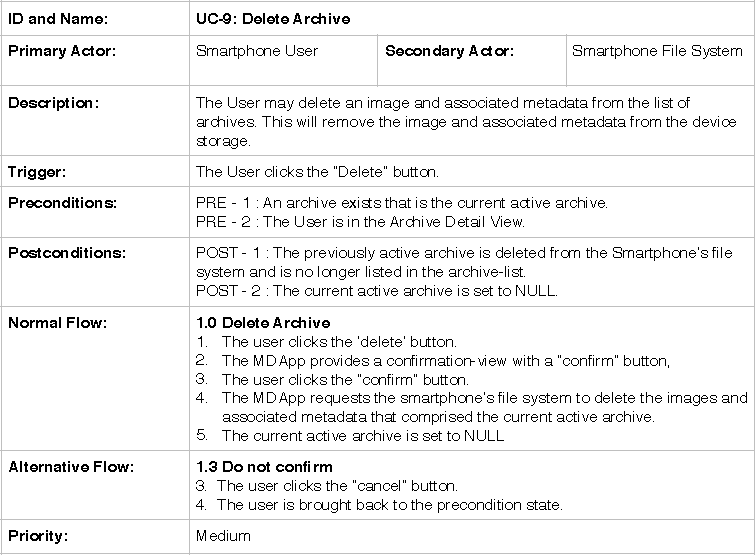
\includegraphics[width=\textwidth]{assets/requirements/uc/usecase_09.pdf}
            \caption{UC-9}
            \label{fig:uc-9}
        \end{table}
        \begin{table}[H]
            \centering
            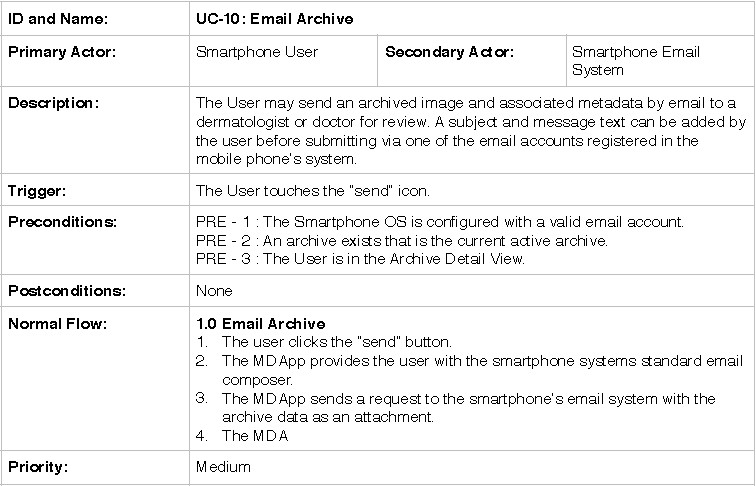
\includegraphics[width=\textwidth]{assets/requirements/uc/usecase_10.pdf}
            \caption{UC-10}
            \label{fig:uc-10}
        \end{table}


\section{Prioritisation}
This project will employ a Single-Criterion Ad-hoc prioritisation classification as opposed to an analytical approach such as the Wiegers prioritisation matrix. The rationale behind this choice is that as a single person development project the determination of weights for benefit, detriment, cost, and risk is an ad-hoc exercise. In a larger project with multiple developers and active stakeholders the time and effort required for a prioritisation assessment according to Wiegers would be advisable.

The following are the prioritisation classes as defined in \cite{9781937538774}:

\begin{itemize}[label={}]

\item \textbf{Mandatory}: A mandatory requirement is a requirement that must be implemented at all costs or else the success of the system is threatened.
\item \textbf{Optional}: An optional requirement is a requirement that does not necessarily need to be implemented. Neglecting a few requirements of this class does not threaten the success of the system.
\item \textbf{Nice-to-have}: Nice-to-have requirements are requirements that do not influence the system’s success if they are not implemented.

\end{itemize}



\section{Requirements}
\section{Prioritized Requirements}

\begin{longtable}{ | l | l | l | l | l | l | l |}
\hline
ID & Priority & Name & Implemented  \\ \hline

REQ-NF-13 & mandatory & Extendability / Updatable & -  \\ \hline
REQ-NF-14 & mandatory & Crossplatform Integration & -  \\ \hline
REQ-F-1 & mandatory & Preview Camera Input & -  \\ \hline
REQ-F-2 & mandatory & Capture Camera Input & -  \\ \hline
REQ-F-3 & mandatory & Border Extraction & -  \\ \hline
REQ-F-4 & mandatory & Browse Images and Results & -  \\ \hline
REQ-F-5 & mandatory & Select Image To View in Detail & -  \\ \hline
REQ-F-6 & mandatory & Border Confirmation & -  \\ \hline
REQ-F-7 & mandatory & Feature Extraction & -  \\ \hline
REQ-F-8 & mandatory & Calculate Risk Assessment & -  \\ \hline
REQ-F-9 & optional & Add/Save/Edit Metadata to Image and Results & -  \\ \hline
REQ-NF-15 & optional & Asynchronous Image Processing & -  \\ \hline
REQ-NF-16 & optional & Good user experience & -  \\ \hline
REQ-F-10 & nice-to-have & Save Image and Associated Data as Archive & -  \\ \hline
REQ-F-11 & nice-to-have & Browse Images and Results from Archive & -  \\ \hline
REQ-F-12 & nice-to-have & Send Image and Associated Data as Email & -  \\ \hline

\caption{Requirement in Detail}
\label{fig:prio_req}
\end{longtable}


\begin{table}[H]
    \begin{tabular}[t]{ | >{\bfseries}l | p{9.5cm} |}

    \hline
    ID
    &  REQ-F-1 \\ \hline

    Name
    & Preview Camera Input \\ \hline

    Description
    &  The system will let the user view a preview of the camera's input in realtime \\ \hline

    Preconditions
    & None \\ \hline

    Acceptance Tests
    & \\ \hline

    Relations
    & UC-1 \\ \hline

    Comments
    &  \\ \hline

    \end{tabular}

    \caption{Functional Requirement 1}
    \label{fig:req_f_1}

\end{table}
\begin{table}[H]
    \begin{tabular}[t]{ | >{\bfseries}l | p{9.5cm} |}

    \hline
    ID
    &  REQ-F-2 \\ \hline

    Name
    & Capture Camera Input \\ \hline

    Description
    &  The system will let the user capture an image from the camera's input. \\ \hline

    Preconditions
    & None \\ \hline

    Acceptance Tests
    & \\ \hline

    Relations
    & UC-1 \\ \hline

    Comments
    &  \\ \hline

    \end{tabular}

    \caption{Functional Requirement 2}
    \label{fig:req_f_2}

\end{table}
\begin{table}[H]
    \begin{tabular}[t]{ | >{\bfseries}l | p{9.5cm} |}

    \hline
    ID
    &  REQ-F-3 \\ \hline

    Name
    & Border Extraction \\ \hline

    Description
    &  The system must be able to calculate the border of a lesion in a captured image. \\ \hline

    Preconditions
    & None \\ \hline

    Acceptance Tests
    & \\ \hline

    Relations
    & UC-2 \\ \hline

    Comments
    &  \\ \hline

    \end{tabular}

    \caption{Functional Requirement 3}
    \label{fig:req_f_3}

\end{table}
\begin{table}[H]
    \begin{tabular}[t]{ | >{\bfseries}l | p{9.5cm} |}

    \hline
    ID
    &  REQ-F-4 \\ \hline

    Name
    & Browse Images and Results \\ \hline

    Description
    &  The system will let the user browse through a list of images. The list will display the status of the images. \\ \hline

    Preconditions
    & None \\ \hline

    Acceptance Tests
    & \\ \hline

    Relations
    &  \\ \hline

    Comments
    &  \\ \hline

    \end{tabular}

    \caption{Functional Requirement 4}
    \label{fig:req_f_4}

\end{table}
\begin{table}[H]
    \begin{tabular}[t]{ | >{\bfseries}l | p{9.5cm} |}

    \hline
    ID
    &  REQ-F-5 \\ \hline

    Name
    & Select Image To View in Detail \\ \hline

    Description
    &  The system will let the user select and view an image as well as the results of completed processes. \\ \hline

    Preconditions
    & None \\ \hline

    Acceptance Tests
    & \\ \hline

    Relations
    &  \\ \hline

    Comments
    &  \\ \hline

    \end{tabular}

    \caption{Functional Requirement 5}
    \label{fig:req_f_5}

\end{table}
\begin{table}[H]
    \begin{tabular}[t]{ | >{\bfseries}l | p{9.5cm} |}

    \hline
    ID
    &  REQ-F-6 \\ \hline

    Name
    & Border Confirmation \\ \hline

    Description
    & The system will let the user confirm that the border of a lesion hat been precisely calculated. \\ \hline

    Preconditions
    &  \\ \hline

    Acceptance Tests
    & \\ \hline

    Relations
    &  \\ \hline

    Comments
    &  \\ \hline

    \end{tabular}

    \caption{Functional Requirement 6}
    \label{fig:req_f_6}

\end{table}
\begin{table}[H]
    \begin{tabular}[t]{ | >{\bfseries}l | p{9.5cm} |}

    \hline
    ID
    &  REQ-F-7 \\ \hline

    Name
    & Feature Extraction \\ \hline

    Description
    & The system must be able to extract relavent features from the isolated lesion image. \\ \hline

    Preconditions
    &  \\ \hline

    Acceptance Tests
    & \\ \hline

    Relations
    &  \\ \hline

    Comments
    &  \\ \hline

    \end{tabular}

    \caption{Functional Requirement 7}
    \label{fig:req_f_7}

\end{table}
\begin{table}[H]
    \begin{tabular}[t]{ | >{\bfseries}l | p{9.5cm} |}

    \hline
    ID
    &  REQ-F-8 \\ \hline

    Name
    & Calculate Risk Assessment \\ \hline

    Description
    & The system must be able to calculate the risk assessment of an lesion being malignant. \\ \hline

    Preconditions
    &  \\ \hline

    Acceptance Tests
    & \\ \hline

    Relations
    &  \\ \hline

    Comments
    &  \\ \hline

    \end{tabular}

    \caption{Functional Requirement 8}
    \label{fig:req_f_8}

\end{table}
\begin{table}[H]
    \begin{tabular}[t]{ | >{\bfseries}l | p{9.5cm} |}

    \hline
    ID
    &  REQ-F-9 \\ \hline

    Name
    & Add/Save/Edit Metadata to Image and Results \\ \hline

    Description
    & The system will allow the user to add or edit metadata associated with the captured image. \\ \hline

    Preconditions
    &  \\ \hline

    Acceptance Tests
    & \\ \hline

    Relations
    &  \\ \hline

    Comments &
        The metadata associated might include the date when the image was captures as well as the location on the body where the lesion is located. The metadata will have the form of a text input field where the user can enter any text. It could be extended, if necessary, with structured data fields.

    \\ \hline

    \end{tabular}

    \caption{Functional Requirement 9}
    \label{fig:req_f_9}

\end{table}
\begin{table}[H]
    \begin{tabular}[t]{ | >{\bfseries}l | p{9.5cm} |}

    \hline
    ID
    &  REQ-F-10 \\ \hline

    Name
    & Save Image and Associated Data as Archive. \\ \hline

    Description
    & The system will allow the user to save images and associated data for reassessment and comparison in the future. \\ \hline

    Preconditions
    &  \\ \hline

    Acceptance Tests
    & \\ \hline

    Relations
    &  \\ \hline

    Comments &

        Storage on a mobile device is a limited resource. Depending on the development strategy chosen, Web App vs Native, the application might not have access to it's own data store. It would be useful to offload data to a cloud or web based storage location.

    \\ \hline

    \end{tabular}

    \caption{Functional Requirement 10}
    \label{fig:req_f_10}

\end{table}
\begin{table}[H]
    \begin{tabular}[t]{ | >{\bfseries}l | p{9.5cm} |}

    \hline
    ID
    &  REQ-F-11 \\ \hline

    Name
    & Browse Images and Results from Archive. \\ \hline

    Description
    & The sytem will allow the user to browse previously saved images and results from the archive. \\ \hline

    Preconditions
    &  \\ \hline

    Acceptance Tests
    & \\ \hline

    Relations
    &  \\ \hline

    Comments
    &  \\ \hline

    \end{tabular}

    \caption{Functional Requirement 11}
    \label{fig:req_f_11}

\end{table}





